\documentclass[11pt, reqno, openany]{memoir}
\usepackage[utf8]{inputenc}
\usepackage[T1]{fontenc}
\usepackage{microtype}
\usepackage[english]{babel}
\usepackage{fullpage}
\usepackage{mathpazo}
\usepackage{marginnote}
\usepackage{amsmath, amsfonts, amssymb, amsthm, mathtools, stmaryrd}
\usepackage{upgreek}
\usepackage{enumerate}
\usepackage[all]{xy}
\usepackage{tikz-cd}
\usepackage{tikz}
\usepackage{comment}
\usepackage{todonotes}
\usepackage{xcolor}
\definecolor{brightmaroon}{rgb}{0.76, 0.13, 0.28}
\usepackage{hyperref}
\hypersetup{
  colorlinks = true,
  linkcolor  = brightmaroon
}
\usepackage[capitalize,nameinlink]{cleveref}
\linespread{1.05}

\vfuzz=14pt % No more shitty ass vbox errors all over the place

\theoremstyle{definition}
\newtheorem{theorem}{Theorem}[section]
\newtheorem{lemma}[theorem]{Lemma}
\newtheorem{axiom}[theorem]{Axiom}
\newtheorem{proposition}[theorem]{Proposition}
\newtheorem{corollary}[theorem]{Corollary}
\newtheorem{definition}[theorem]{Definition}
\newtheorem{remark}[theorem]{Remark}
\newtheorem{example}[theorem]{Example}
\newtheorem{notation}[theorem]{Notation}

%\parskip=5pt plus 1pt

% symbols
\renewcommand{\qedsymbol}{\(\blacklozenge\)}
\renewcommand{\leq}{\leqslant}
\renewcommand{\geq}{\geqslant}
\renewcommand{\setminus}{\smallsetminus}
\newcommand{\dual}{\vee}

\DeclareMathOperator{\Hom}{Hom}
\DeclareMathOperator{\Obj}{Obj}
\DeclareMathOperator{\Mor}{Mor}
\DeclareMathOperator{\End}{End}
\DeclareMathOperator{\Aut}{Aut}
\DeclareMathOperator{\Id}{id}
\DeclareMathOperator{\im}{im}
\DeclareMathOperator{\dom}{dom}
\DeclareMathOperator{\codom}{codom}
\DeclareMathOperator{\rank}{rank}
\DeclareMathOperator{\coker}{coker}
\DeclareMathOperator{\Int}{Int}
\DeclareMathOperator{\Ext}{Ext}
\DeclareMathOperator{\Tr}{tr}
\DeclareMathOperator{\Sym}{Sym}
\DeclareMathOperator{\Char}{char}
\DeclareMathOperator{\sign}{sign}

% arrows
\newcommand{\op}{\mathrm{op}}
\newcommand{\isoto}{\xrightarrow{\raisebox{-.5ex}[0ex][0ex]{$\sim$}}}
\newcommand{\To}{\Rightarrow}
\newcommand{\mono}{\hookrightarrow}
\newcommand{\epi}{\twoheadrightarrow}
\newcommand{\cat}{\mathcal}
\newcommand{\iso}{\simeq} % changed from simeq

\newcommand{\Z}{\mathbf{Z}}
\newcommand{\N}{\mathbf{N}}
\newcommand{\Q}{\mathbf{Q}}
\newcommand{\CC}{\mathbf{C}}
\newcommand{\R}{\mathbf{R}}

% cats
\newcommand{\Set}{{\cat{S}\textit{et}}}
\newcommand{\Vect}{{\cat{V}\textit{ect}}}
\newcommand{\FinVect}{{\cat{F}\textit{in}\cat{V}\textit{ect}}}
\newcommand{\Top}{{\cat{T}\textit{op}}}
\newcommand{\Grp}{{\cat{G}\textit{rp}}}
\newcommand{\Ab}{{\cat{A}\textit{b}}}
\newcommand{\Graph}{{\cat{G}\textit{raph}}}
\newcommand{\Rng}{{\cat{R}\textit{ing}}}

\title{Algebra \& Categories --- An Introduction}
\author{Luiz G. Mugnaini A.}
\date{Last modification: \today}

\begin{document}
\maketitle
\tableofcontents
\listoftodos


\newcommand{\onlyinsubfile}[1]{#1}
\newcommand{\notinsubfile}[1]{}

\author{Luiz G. Mugnaini A.}
\date{Last modification: \today}
\title{Deep Dive}

\begin{document}

\renewcommand{\onlyinsubfile}[1]{}
\renewcommand{\notinsubfile}[1]{#1}

\frontmatter

% \begin{titlingpage}
% Peter Haine stuff!
\DeclareFixedFont{\titlefont}{T1}{ppl}{b}{n}{0.6in}
\DeclareFixedFont{\subtitlefont}{T1}{ppl}{b}{n}{0.35in}
\DeclareFixedFont{\subsubtitlefont}{T1}{ppl}{b}{n}{0.2in}
\newgeometry{left=0.6in, right=0.6in,top=0in, bottom=0in}
\afterpage{\aftergroup\changegeometry}
\pagecolor{black}\afterpage{\nopagecolor}

\thispagestyle{empty}
\begin{center}
\begin{tikzpicture}
\node[
inner sep=0pt,
outer sep=0pt
]{
 \makebox[\textwidth]{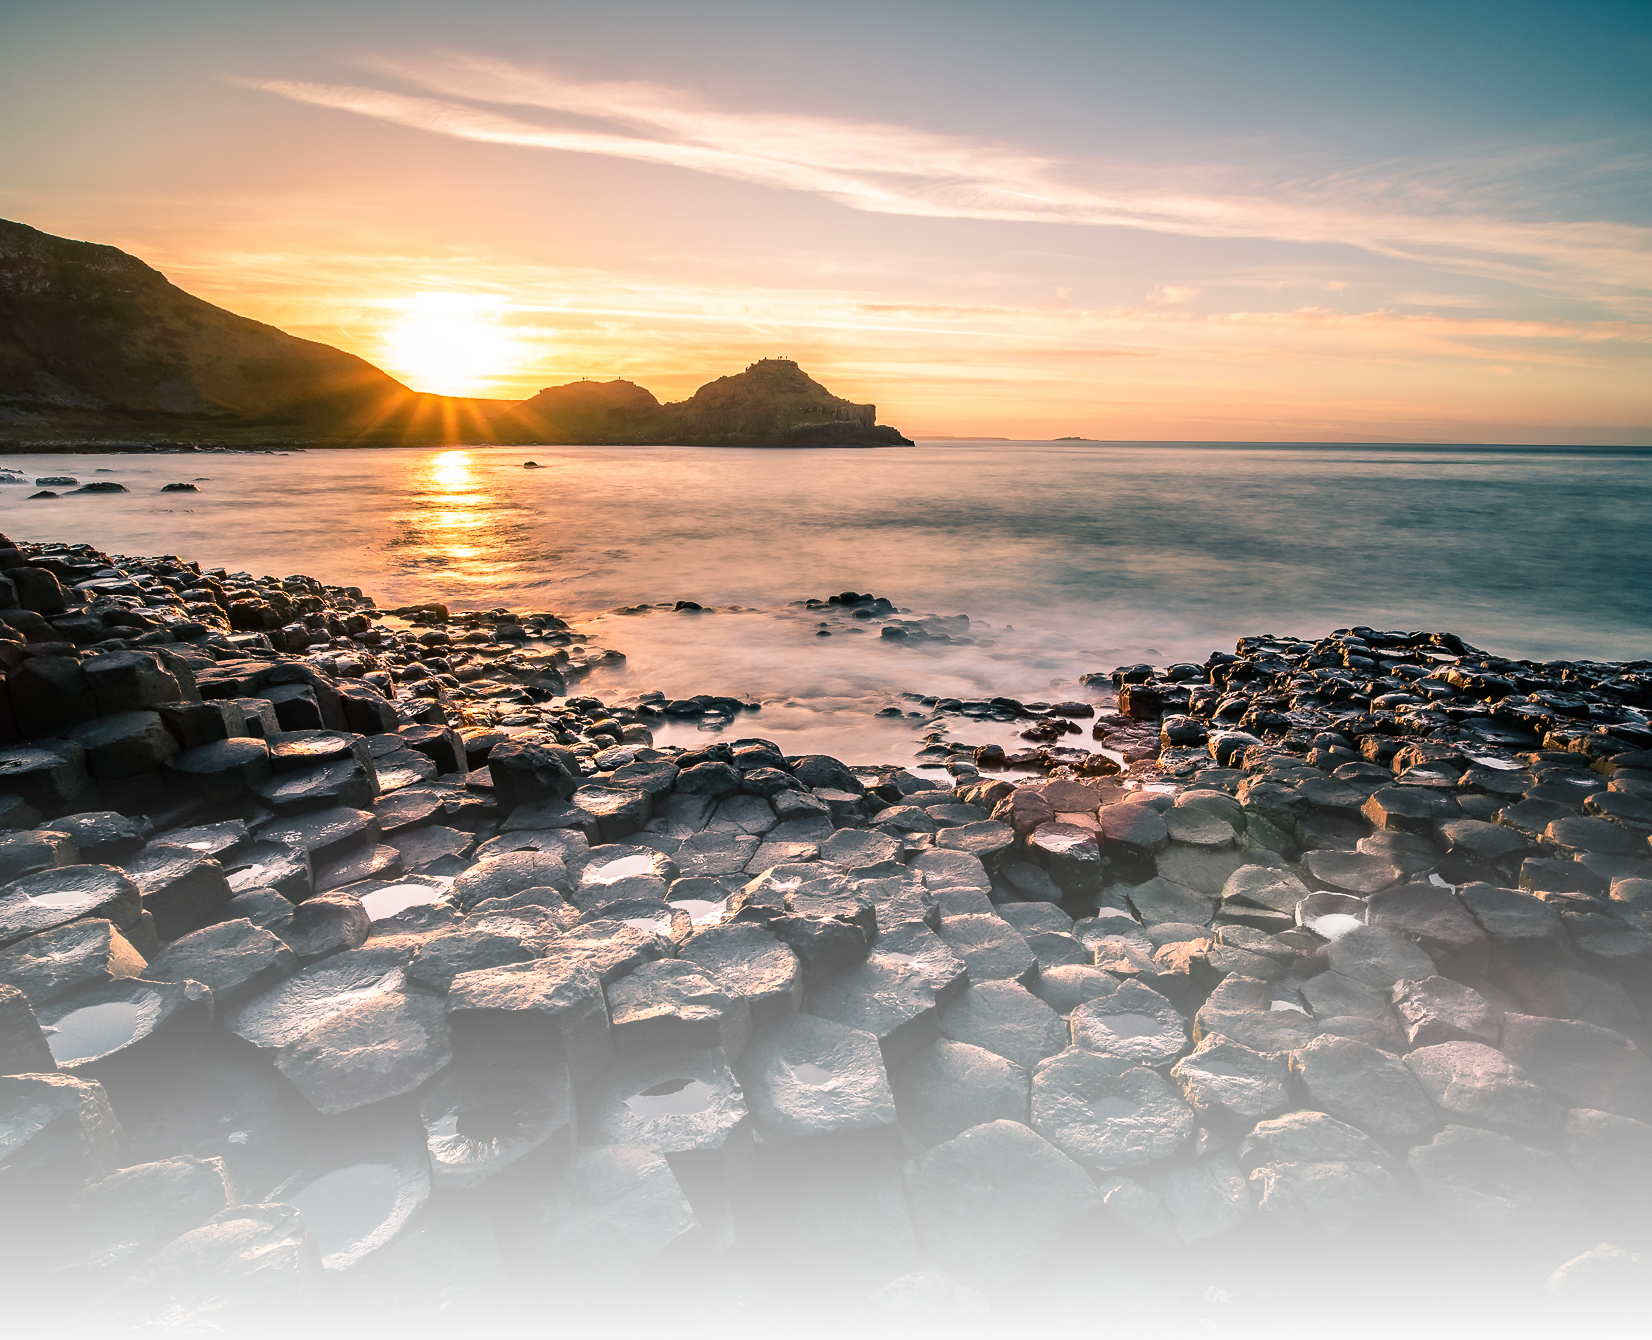
\includegraphics[width=635pt]{src/hexagons}}
};
\end{tikzpicture}
\vspace{1cm}

\textcolor{white}{
\titlefont Deep-Dive \\[0.3cm]
\subtitlefont Studies Into Mathematics\\[0.75cm]
\subsubtitlefont Luiz G. Mugnaini A.\\[0.75cm]Last Modification: \today
}
\end{center}
\newpage
\end{titlingpage}

%%% Local Variables:
%%% mode: latex
%%% TeX-master: "../deep-dive"
%%% End:

\maketitle

\tableofcontents
\listoftodos

% \pagestyle{plain}

% \chapter{Preface}

% First of all I should stress that the title page template was taken from the
% beautiful book~\cite{Haine21DiffCoho} by P. Haine et al.~--- the whole credit
% should be given to them. The following text is a compilation of notes for my
% studies in mathematics, that being said, it is clear that the collection of
% mathematical and linguistic errors is non-empty. My main references are
% \begin{itemize}\setlength\itemsep{0em}
% \item Category Theory:~\cite{Rie16} and~\cite{Shap06}.
% \item Algebra:~\cite{Yu89},~\cite{Kim20},~\cite{Aluf09} and~\cite{Lang93}.
% \item Topology:~\cite{Lee11},~\cite{Tai20},~\cite{Mun00} and~\cite{Eng89}.
% \item Differential Structures:~\cite{Zor15},~\cite{Zor16},~\cite{Rud76}
%   and~\cite{Jost06}.
% \item Combinatorics:~\cite{Die16}.
% \end{itemize}

\mainmatter

% NOTE: the spacing correction in the part titles is needed because latex
% handles absolutely poorly the spacing between the roman numbers and the title

\part{Category Theory}

\subfile{src/category-theory/main-categories}

% \part{Algebra}

% \subfile{src/algebra/linalg/main-linalg}
% \subfile{src/algebra/group/main-group}
% \subfile{src/algebra/rings-and-modules/main-rings-and-modules}

% \part{~~Combinatorics}

% \subfile{src/combinatorics/main-combinatorics}

\part{~~Classical Topology}

\subfile{src/topology/classical-topology/main-classical-topology}

\part{~~Homotopy Theory}

\subfile{src/topology/homotopy-theory/main-htpy}

% \part{~~Manifold Theory}

% \subfile{src/differentiable/manifold/main-manifold}

% \part{~~~Analysis}

% \subfile{src/differentiable/functional-analysis/main-functional-analysis}

% \part{~~~Machine Learning}

% \subfile{src/statnprob/main-statnprob}

% \appendix

% \part{~~~~Appendix}

% \subfile{src/appendix/main-appendix}
% \subfile{src/appendix/papers/main-papers}

% \printbibliography

\end{document}
%%% Local Variables:
%%% mode: latex
%%% TeX-master: t
%%% End:
